In this section, we provide additional details on the thermal model utilized by the proposed UQ framework at Stage~3, \sref{thermal-model}. We use the widespread model based on Fourier's heat equation, which, after a proper spacial discretization, leads to the following system of DAEs:
\begin{subnumcases}{\elabel{fourier-system-original}}
  \mC \: \frac{d\vTI(\t)}{d\t} + \mG \: \vTI(\t) = \mM \: \vP(\t) \elabel{fourier-original} \\
  \vTO(\t) = \mM^T \vTI(\t) + \vTO_\amb
\end{subnumcases}
where the number of differential equations is equal to the number of thermal nodes, $\nnodes$; $\mC, \mG \in \real^{\nnodes \times \nnodes}$ are a diagonal matrix of the thermal capacitance and a symmetric, positive-definite matrix of the thermal conductance, respectively; $\vTI \in \real^\nnodes$ is the vector of the difference between the temperature of the thermal nodes and the ambient temperature; $\vP \in \real^\nprocs$ and $\mM \in \real^{\nnodes \times \nprocs}$ are the input vector of power and its mapping matrix to the thermal nodes; $\vTO \in \real^\nprocs$ is the temperature vector of the processing elements, and $\vTO_\amb \in \real^\nprocs$ is the vector of the ambient temperature. For convenience, we perform an auxiliary transformation of \eref{fourier-system-original} using \cite{ukhov2012}
\begin{equation*}
  \vX = \mC^\frac{1}{2} \vTI, \hspace{1em} \mA = -\mC^{-\frac{1}{2}} \mG \mC^{-\frac{1}{2}}, \hspace{1em} \text{and} \hspace{1em} \mB = \mC^{-\frac{1}{2}} \mM
\end{equation*}
and obtain the system in \eref{fourier-system}, which is rewritten in the stochastic form, where the coefficient matrix $\mA$ preserves the symmetry and positive-definiteness of $\mG$. In general, the differential part in \eref{fourier-system}, or equally in \eref{fourier-system-original}, is nonlinear due to the source term $\vP(\t)$ since we do not make any assumptions about its structure (see the discussion in \sref{power-model}). Therefore, there are no closed-form solutions to the system.

The time intervals $\{ \dt_i \}_{i = 1}^\nsteps$ of the power sampling (see \sref{problem-formulation}) are assumed to be short enough such that the total power can be approximated as constant within one interval. In this case, \eref{fourier-de} is a system of linear differential equations that can be solved analytically. The solution is \cite{ukhov2012}
\begin{equation} \elabel{ode-solution}
  \vX(\t) = \mCF(\t) \: \vX(0) + \mCS(\t) \: \vP(0)
\end{equation}
where $\t$ is restricted to one time interval, $\vP(0)$ is the power dissipation at the beginning of the time interval with respect to the corresponding temperature,
\begin{align*}
  & \mCF(\t) = e^{\mA \t} \in \real^{\nnodes \times \nnodes}, \text{ and} \\
  & \mCS(\t) = \mA^{-1} (e^{\mA \t} - \mI) \: \mB \in \real^{\nnodes \times \nprocs}.
\end{align*}
The procedure is to be repeated for all time intervals $\{ \dt_k \}_{k=1}^\nsteps$ starting from the initial temperature, which, without loss of generality, is assumed to be equal to the ambient temperature. It is worth being noted that, when the power profile is evenly sampled, the coefficient matrices $\mCF(\t)$ and $\mCS(\t)$ are constant and can be efficiently computed using the technique proposed in \cite{ukhov2012}.  Finally, introducing the dependency on $\o \in \outcomes$, we obtain the recurrence in \eref{recurrence}.
\begin{figure}
  \centering
  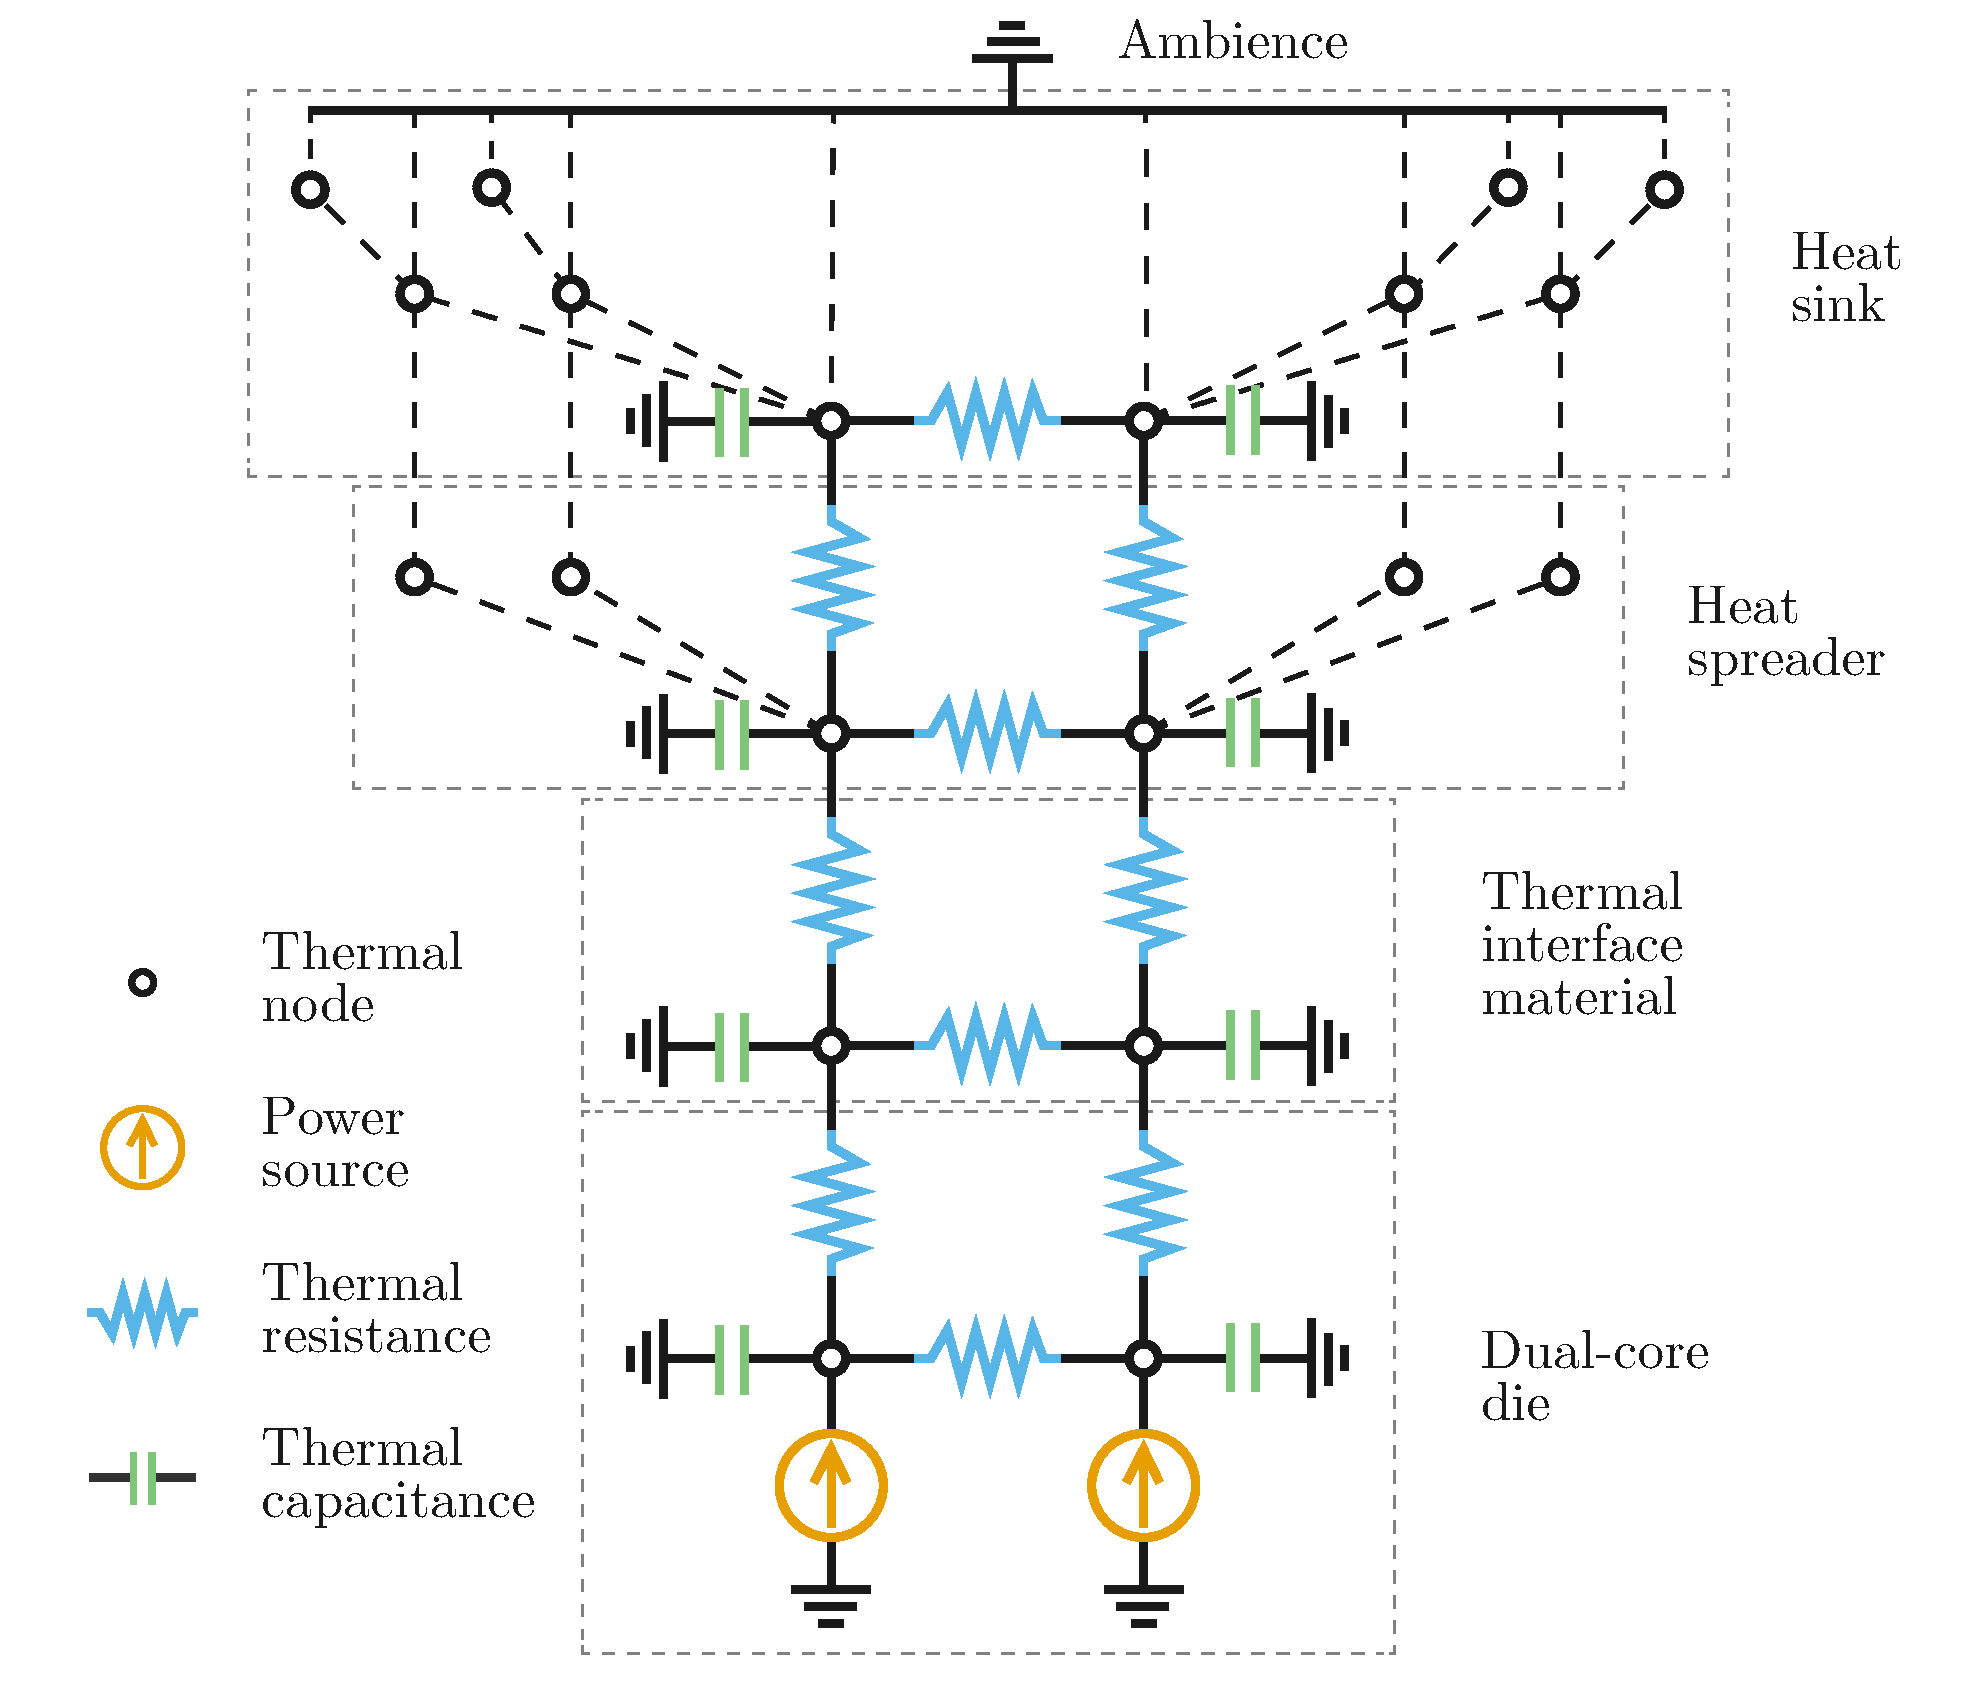
\includegraphics[width=\linewidth]{include/assets/circuit.pdf}
  \vspace{-1.0em}
  \caption{A simplified thermal RC circuit of a dual-core platform with a three-layer thermal package.}
  \flabel{circuit}
  \vspace{-1.5em}
\end{figure}

